\documentclass[12pt,a4paper]{article}
\usepackage[T1]{fontenc}
\usepackage[spanish,es-nodecimaldot]{babel}
\usepackage{tgtermes}
\usepackage{newtxmath}
\usepackage{amsmath}
\usepackage{textcomp}
\usepackage{graphicx}
\usepackage{geometry}
\usepackage{xcolor}
\usepackage{setspace}
\usepackage{titlesec}
\usepackage{tocloft}
\usepackage{fancyhdr}
\usepackage{enumitem}
\usepackage{hyperref}

\geometry{margin=2.5cm}

\definecolor{AzulPrincipal}{HTML}{0B2D4D}
\definecolor{AzulSecundario}{HTML}{1F5F8B}
\definecolor{OroAcento}{HTML}{C9A227}
\definecolor{GrisTexto}{HTML}{444444}

\hypersetup{
    colorlinks=true,
    linkcolor=black,
    urlcolor=black,
    citecolor=black,
    pdftitle={Plantilla de Informe},
    pdfauthor={Tu Nombre}
}

\setlength{\parindent}{1.25cm}
\setlength{\parskip}{0.25em}
\onehalfspacing

\setlist[itemize]{leftmargin=2.8em, labelsep=0.8em, topsep=0.35em, itemsep=0.2em}
\setlist[enumerate]{leftmargin=1.7em, topsep=0.35em, itemsep=0.2em}

\titleformat{\section}[hang]{\fontsize{18pt}{22pt}\selectfont\normalfont\color{black}}{\thesection.}{0.8em}{}
\titleformat{\subsection}[hang]{\fontsize{14pt}{17pt}\selectfont\normalfont\color{black}}{\thesubsection}{0.8em}{}

\renewcommand{\cftsecfont}{\normalfont}
\renewcommand{\cftsecpagefont}{\normalfont}
\renewcommand{\cftsubsecfont}{\normalfont}
\renewcommand{\cftsubsecpagefont}{\normalfont}
\renewcommand{\cftsecleader}{\cftdotfill{\cftdotsep}}
\renewcommand{\cftsubsecleader}{\cftdotfill{\cftdotsep}}
\renewcommand{\contentsname}{Índice}
\renewcommand{\cfttoctitlefont}{\hfill\normalfont\fontsize{18pt}{22pt}\selectfont}
\renewcommand{\cftaftertoctitle}{\hfill}

\titlespacing*{\section}{0pt}{1.1em}{0.55em}
\titlespacing*{\subsection}{0pt}{0.9em}{0.35em}

\setlength{\headheight}{30pt}

\pagestyle{fancy}
\fancyhf{}
\lhead{\small\textcolor{black!65}{\Laboratorio: \Tema}}
\rhead{}
\cfoot{\small\textcolor{black}{\thepage}}
\renewcommand{\headrulewidth}{0.4pt}
\renewcommand{\headrule}{\hbox to\headwidth{\color{black!65}\leaders\hrule height \headrulewidth\hfill}}
\renewcommand{\footrulewidth}{0pt}

\providecommand{\Universidad}{UNIVERSIDAD NACIONAL DE INGENIERÍA}
\providecommand{\Facultad}{FACULTAD DE CIENCIAS}
\providecommand{\Escuela}{ESCUELA DE FÍSICA}
\providecommand{\Curso}{CIRCUITOS ELÉCTRICOS ANALÓGICOS}
\providecommand{\Seccion}{SECCIÓN A}
\providecommand{\NumeroLaboratorio}{X}
\providecommand{\Laboratorio}{LABORATORIO N\textdegree{} \NumeroLaboratorio}
\providecommand{\Tema}{TÍTULO DE LA PRÁCTICA}
\providecommand{\RutaLogo}{logo.PNG}
\providecommand{\IntegrantesBloque}{%
\begin{enumerate}[leftmargin=1.8em,label=\arabic*.]
    \item Integrante 1 -- código
    \item Integrante 2 -- código
\end{enumerate}}
\providecommand{\FechaRealizacion}{Fecha de realización: dd de mes de aaaa - hh:mm}
\providecommand{\Ciudad}{LIMA - PERU}

\newcommand{\ConfigurarInforme}[3]{%
    \renewcommand{\NumeroLaboratorio}{#1}%
    \renewcommand{\Tema}{#2}%
    \renewcommand{\FechaRealizacion}{#3}%
}

\newcommand{\ConfigurarIntegrantes}[1]{%
    \renewcommand{\IntegrantesBloque}{#1}%
}

\providecommand{\tituloSeccion}[1]{\section{#1}}

\providecommand{\makeInformePortada}{%
\begin{titlepage}
    \thispagestyle{empty}
    \vspace*{0.65cm}
    \begin{center}
        {\Large\bfseries\color{OroAcento} \Universidad}\par
        \vspace{0.45cm}
        {\Large\bfseries\color{AzulPrincipal} \Facultad}\par
        \vspace{0.25cm}
        {\Large\bfseries\color{AzulPrincipal} \Escuela}\par
    \end{center}

    \vspace{0.1cm}
    \begin{center}
        \includegraphics[width=0.4\textwidth]{\RutaLogo}%
    \end{center}

    \vspace{0.01cm}
    \begin{center}
        {\Large\bfseries\color{AzulPrincipal} \Curso}\par
        \vspace{0.35cm}
        {\Large\bfseries\color{red} \Seccion}\par
    \end{center}

    \vspace{0.1cm}
    \begin{center}
        {\large\bfseries \Laboratorio: \Tema}\par
    \end{center}

    \vspace{0.55cm}
    \noindent{\large\textbf{INTEGRANTES DE LA MESA:} 2}\par
    \vspace{0.35cm}
    \begingroup
    \leftskip=1.15cm
    \rightskip=1.15cm
    \parindent=0pt
    \IntegrantesBloque
    \endgroup

    \vspace{0.55cm}
    \begin{center}
        {\FechaRealizacion}\par
    \end{center}

    \vfill

    \begin{center}
        {\large\bfseries \Ciudad}
    \end{center}
\end{titlepage}
}
\usepackage{tikz}
\usepackage{pgfplots}
\pgfplotsset{compat=1.18}
\renewcommand{\RutaLogo}{../../PLANTILLA/logo.PNG}
\graphicspath{{Imagenes/}}
\ConfigurarInforme{9}{Regulador de voltaje}{Fecha de realización del Laboratorio N\textdegree{}9: 16 de Mayo del 2026}

% Inicio del informe
\begin{document}
\makeInformePortada
\setcounter{page}{1}
\tableofcontents
\newpage

\tituloSeccion{Objetivos}
\subsection{Objetivo General}
Estudiar el funcionamiento del regulador de voltaje integrado LM7805.

\subsection{Objetivos Específicos}
\begin{enumerate}
\item Comprobar la salida en voltaje del regulador integrado LM7805.
\item Ajustar el valor de la resistencia de carga en un circuito con un regulador de voltaje para establecer un voltaje de salida específico.
\end{enumerate}

\tituloSeccion{Fundamento teórico}

Los reguladores de voltaje son dispositivos utilizados para mantener una tensión de salida prácticamente constante frente a variaciones en la tensión de entrada o en la carga. En una fuente de alimentación regulada, el regulador reduce el rizado de una señal previamente rectificada y filtrada, proporcionando una salida estable.

Los reguladores de voltaje se clasifican principalmente en reguladores serie y reguladores paralelo. En un regulador serie, el elemento regulador se coloca en serie con la carga y ajusta la caída de tensión para compensar variaciones en la entrada o en la corriente de carga. En un regulador paralelo, el elemento regulador se conecta en derivación con la carga y desvía corriente hacia tierra para mantener estable el voltaje.

\subsection{Reguladores de voltaje integrados}

Los reguladores integrados incorporan en un solo circuito los elementos necesarios para la regulación y protección del sistema. Entre sus ventajas destacan la simplicidad de uso, la reducción del número de componentes externos y la inclusión de protecciones térmicas y de corriente.

Los reguladores de la serie 78XX proporcionan tensiones positivas fijas. El número que acompaña al dispositivo indica el voltaje nominal de salida; por ejemplo, el 7805 entrega $+5\,\text{V}$ y el 7812 entrega $+12\,\text{V}$. Estos dispositivos poseen tres terminales: entrada (IN), salida (OUT) y tierra (GND).

Para garantizar estabilidad y disminuir el ruido de alta frecuencia, normalmente se colocan condensadores en la entrada y salida del regulador.

\subsection{Regulación de carga}

En una fuente regulada ideal, el voltaje de salida sin carga y con carga deberían ser iguales. Sin embargo, en condiciones reales existe una pequeña variación debido a la corriente suministrada a la carga. Experimentalmente, el porcentaje de regulación se calcula mediante:

\begin{equation}
\%\,\text{regulación}=
\frac{V_{out}-V_{out_L}}{V_{out}}\cdot100\%.
\label{eq:regulacion}
\end{equation}

donde $V_{out}$ es el voltaje de salida sin carga y $V_{out_L}$ es el voltaje de salida con carga. Mientras menor sea este porcentaje, mejor será la regulación de la fuente.

\subsection{Reguladores ajustables}

Además de los reguladores de salida fija, existen reguladores ajustables como el LM317, cuya tensión de salida puede establecerse mediante una red resistiva externa. La relación entre la tensión de salida y las resistencias está dada por:

\begin{equation}
V_{out}=V_{ref}\left(1+\frac{R_2}{R_1}\right)+I_{adj}R_2,
\label{eq:voltaje_salida}
\end{equation}

donde $V_{ref}$ es la tensión de referencia interna del regulador (aproximadamente $1.25\,\text{V}$), $R_1$ y $R_2$ son las resistencias de ajuste, e $I_{adj}$ es la corriente del pin de ajuste.

En aplicaciones prácticas, el término $I_{adj}R_2$ suele ser pequeño y frecuentemente puede despreciarse. De esta manera, el voltaje de salida depende principalmente de la relación entre las resistencias $R_1$ y $R_2$.
\tituloSeccion{Materiales e indicaciones}
\begin{itemize}
	\item Multímetro: Instrumento de medición utilizado para verificar los valores de resistencia de los componentes, así como para medir voltajes en el circuito. 
    \item Regulador de voltaje LM7805: Es un regulador lineal de voltaje positivo que proporciona una salida fija de 5 V. Para su uso, se debe conectar el pin de entrada a la fuente de voltaje, el pin de tierra a tierra y el pin de salida al circuito que se desea alimentar.
    \item Resistencias: Son componentes que limitan el flujo de corriente en un circuito. Para su uso, se deben identificar sus valores utilizando el código de colores o un multímetro, y conectarlas en el circuito según sea necesario.
    \item Protoboard: Es una placa de pruebas que permite realizar conexiones temporales sin necesidad de soldar. Para su uso, se deben insertar los componentes en las filas y columnas correspondientes, y realizar las conexiones utilizando cables de puente.
\end{itemize}

\newpage
\tituloSeccion{Procedimiento Experimental}
\subsection{Paso 1}
\begin{enumerate}
    \item Montamos el circuito de la figura \ref{fig:circuito1} con el LM7805 y medimo la tensión de salida $V_{out}$ para diferentes valores de la tensión de entrada $V_{in}$.
    \begin{figure}[H]
        \centering
        
\includegraphics[width=0.5\linewidth]{imagen1.png}
        \caption{Circuito con regulador LM7805 para medir $V_{out}$ vs $V_{in}$. [2]}
        \label{fig:circuito1}
    \end{figure}
    \item Registramos los datos obtenidos en la tabla \ref{tab:tabla1} y graficamos $V_{out}$ en función de $V_{in}$ para observar el comportamiento del regulador.
\end{enumerate}

\subsection{Paso 2}
\begin{enumerate}
    \item Montamos el circuito regulador ajustable con la configuración de la figura \ref{fig:circuito-potenciometro}, usamos la fórmula \ref{eq:voltaje_salida} para calcular $V_{out}$ en función de $R_2$ y $I_{aj}$,
    donde $I_{aj}$ es la corriente que sale de la pata 2 del regulador LM7805.
    \begin{figure}[H]
        \centering
        
\includegraphics[width=0.5\linewidth]{imagen2.png}
        \caption{Circuito regulador con potenciómetro. [2]}
        \label{fig:circuito-potenciometro}
    \end{figure}
    \item Se fijó $V_{in}=20$. Por otro lado, se varió el valor de $R_2$ y se midió experimentalmente $I_{aj}$ para obtener diferentes valores de $V_{out}$ y se registraron los datos en la tabla \ref{tab:tabla2}. Se calculó el porcentaje de error entre el valor calculado de $V_{out}$ usando la fórmula y el valor medido con el multímetro.
    \item Con $V_{in}$ fijo, se ajustó $R_2$ para obtener $V_{out}\approx 8\,$V, luego se disminuyó el voltaje de entrada $V_{in}$ y se determinó el rango para el cual $V_{out}$ se mantiene fijo. Los datos obtenidos se registraron en la tabla \ref{tab:tabla3}.
\end{enumerate}

\subsection{Paso 3}
\begin{enumerate}
    \item Le agregamos al circuito anterior una resistencia de carga variable $R_L$ en paralelo y en serie a esta una resistencia de protección de $467,5 \Omega$ como en la figura \ref{fig:circuito-carga}. Se midió la corriente $I_L$ que circula por $R_L$ y el voltaje en $R_L$ para diferentes valores de $R_L$. Con estos datos se calculó el porcentaje de regulación según la fórmula \ref{eq:regulacion}.
    \begin{figure}[H]
        \centering
        
\includegraphics[width=0.5\linewidth]{Imagen3.png}
        \caption{Circuito con resistencia de carga variable $R_L$. [2]}
        \label{fig:circuito-carga}
    \end{figure}
	\item Los datos obtenidos se registraron en la tabla \ref{tab:tabla4}.
\end{enumerate}

\tituloSeccion{Análisis de datos}

\subsection{Paso 1}
\begin{table}[H]
	\centering
	\fontsize{10pt}{12pt}\selectfont
	\renewcommand{\arraystretch}{1.2}
	\setlength{\tabcolsep}{6pt}
	{\begin{tabular}{|C{4.5cm}|C{4.5cm}|}
	\hline
	$V_{in}$ (V) & $V_{out}$ (V) \\
	\hline
	2,9 $\pm$ 0,1 & 0,1 $\cdot 10^{-3}$ $\pm$ 0,001 \\
	\hline
	4,1 $\pm$ 0,1 & 54,0 $\cdot 10^{-3}$ $\pm$ 0,001 \\
	\hline
	4,9 $\pm$ 0,1 & 3,412 $\pm$ 0,001 \\
	\hline
	5,9 $\pm$ 0,1 & 4,450 $\pm$ 0,001 \\
	\hline
	7,1 $\pm$ 0,1 & 4,988 $\pm$ 0,001 \\
	\hline
	8,1 $\pm$ 0,1 & 4,959 $\pm$ 0,001 \\
	\hline
	8,9 $\pm$ 0,1 & 4,938 $\pm$ 0,001 \\
	\hline
	10,1 $\pm$ 0,1 & 4,940 $\pm$ 0,001 \\
	\hline
	11,2 $\pm$ 0,1 & 4,946 $\pm$ 0,001 \\
	\hline
	12,1 $\pm$ 0,1 & 4,948 $\pm$ 0,001 \\
	\hline
	13,1 $\pm$ 0,1 & 4,931 $\pm$ 0,001 \\
	\hline
	14,0 $\pm$ 0,1 & 4,934 $\pm$ 0,001 \\
	\hline
	15,2 $\pm$ 0,1 & 4,941 $\pm$ 0,001 \\
	\hline
	16,0 $\pm$ 0,1 & 4,945 $\pm$ 0,001 \\
	\hline
	16,9 $\pm$ 0,1 & 4,954 $\pm$ 0,001 \\
	\hline
	18,2 $\pm$ 0,1 & 4,960 $\pm$ 0,001 \\
	\hline
	19,0 $\pm$ 0,1 & 4,960 $\pm$ 0,001 \\
	\hline
	20,1 $\pm$ 0,1 & 4,954 $\pm$ 0,001 \\
	\hline
	\end{tabular}}
	\caption{Mediciones de $V_{out}$ vs $V_{in}$.}
	\label{tab:tabla1}
\end{table}

Como se ve en la siguiente gráfica, el voltaje umbral de operación es aproximadamente $4,5\,$V, por debajo del cual $V_{out}$ cae rápidamente a valores cercanos a cero. A partir de ese punto, $V_{out}$ se mantiene prácticamente constante en torno a $5\,$V a medida que $V_{in}$ aumenta, lo que confirma el funcionamiento de regulación del LM7805.

El voltaje de salida nominal en la región de regulación es de $5\,$V, aunque en las mediciones se observa una valor real con ligera variación (en torno a $4,94\,$V--$4,96\,$V) que puede atribuirse a la tolerancia del regulador o las características de la fuente utilizada. La curva muestra claramente la transición entre la región de no regulación (donde $V_{out}$ sigue aproximadamente a $V_{in}$) y la región de regulación (donde $V_{out}$ se estabiliza).

\begin{figure}[H]
	\centering
	\begin{tikzpicture}
	\begin{axis}[
		width=0.9\linewidth,
		xlabel={$V_{out}$ (V)},
		ylabel={$V_{in}$ (V)},
		grid=both,
		grid style={line width=.1pt, draw=gray!20},
		major grid style={line width=.2pt,draw=gray!50},
		xmin=0, xmax=5.5,
		ymin=2, ymax=21,
		xtick={0,0.5,1,1.5,2,2.5,3,3.5,4,4.5,5},
		ytick={2,4,6,8,10,12,14,16,18,20},
		tick align=outside
	]
	\addlegendentry{Experimental (barras x5 para visualizacion)}

	\addplot[
		black,
		only marks,
		mark=none,
		forget plot,
		error bars/.cd,
			x dir=both,
			x explicit,
			error bar style={line width=0.2pt},
			error mark=-,
			error mark options={mark size=4pt, line width=0.2pt}
	]
	coordinates {
		(0.0001,2.9) +- (0.005,0)
		(0.054,4.1) +- (0.005,0)
		(3.412,4.9) +- (0.005,0)
		(4.450,5.9) +- (0.005,0)
		(4.988,7.1) +- (0.005,0)
		(4.959,8.1) +- (0.005,0)
		(4.938,8.9) +- (0.005,0)
		(4.940,10.1) +- (0.005,0)
		(4.946,11.2) +- (0.005,0)
		(4.948,12.1) +- (0.005,0)
		(4.931,13.1) +- (0.005,0)
		(4.934,14.0) +- (0.005,0)
		(4.941,15.2) +- (0.005,0)
		(4.945,16.0) +- (0.005,0)
		(4.954,16.9) +- (0.005,0)
		(4.960,18.2) +- (0.005,0)
		(4.960,19.0) +- (0.005,0)
		(4.954,20.1) +- (0.005,0)
	};
	\addplot[
		black,
		only marks,
		mark=none,
		forget plot,
		error bars/.cd,
			y dir=both,
			y explicit,
			error bar style={line width=0.2pt},
			error mark=|,
			error mark options={mark size=4pt, line width=0.2pt}
	]
	coordinates {
		(0.0001,2.9) +- (0,0.5)
		(0.054,4.1) +- (0,0.5)
		(3.412,4.9) +- (0,0.5)
		(4.450,5.9) +- (0,0.5)
		(4.988,7.1) +- (0,0.5)
		(4.959,8.1) +- (0,0.5)
		(4.938,8.9) +- (0,0.5)
		(4.940,10.1) +- (0,0.5)
		(4.946,11.2) +- (0,0.5)
		(4.948,12.1) +- (0,0.5)
		(4.931,13.1) +- (0,0.5)
		(4.934,14.0) +- (0,0.5)
		(4.941,15.2) +- (0,0.5)
		(4.945,16.0) +- (0,0.5)
		(4.954,16.9) +- (0,0.5)
		(4.960,18.2) +- (0,0.5)
		(4.960,19.0) +- (0,0.5)
		(4.954,20.1) +- (0,0.5)
	};
	\addplot[
		color=blue,
		thick,
		mark=*,
		mark options={fill=blue, draw=blue},
		mark size=2.5pt
	]
	coordinates {
		(0.0001,2.9) +- (0.005,0.5)
		(0.054,4.1) +- (0.005,0.5)
		(3.412,4.9) +- (0.005,0.5)
		(4.450,5.9) +- (0.005,0.5)
		(4.988,7.1) +- (0.005,0.5)
		(4.959,8.1) +- (0.005,0.5)
		(4.938,8.9) +- (0.005,0.5)
		(4.940,10.1) +- (0.005,0.5)
		(4.946,11.2) +- (0.005,0.5)
		(4.948,12.1) +- (0.005,0.5)
		(4.931,13.1) +- (0.005,0.5)
		(4.934,14.0) +- (0.005,0.5)
		(4.941,15.2) +- (0.005,0.5)
		(4.945,16.0) +- (0.005,0.5)
		(4.954,16.9) +- (0.005,0.5)
		(4.960,18.2) +- (0.005,0.5)
		(4.960,19.0) +- (0.005,0.5)
		(4.954,20.1) +- (0.005,0.5)
	};

	\end{axis}
	\end{tikzpicture}
	\caption{Gráfico de $V_{out}$ vs $V_{in}$.}
	\label{fig:vout_vs_vin}
\end{figure}

\textbf{ANÁLISIS:} El gráfico muestra claramente la característica de regulación del LM7805. Para $V_{in}$ por debajo de aproximadamente $4,5\,$V, el regulador no puede mantener la salida en $5\,$V y $V_{out}$ cae rápidamente. A partir de ese punto, $V_{out}$ se estabiliza cerca de $5\,$V a medida que $V_{in}$ aumenta, lo que confirma el funcionamiento esperado del regulador. La ligera variación en el valor de $V_{out}$ en la región de regulación puede atribuirse a la tolerancia del componente o a las propias características de la fuente utilizada.

\subsection{Paso 2}

\begin{table}[H]
	\centering
	\fontsize{10pt}{12pt}\selectfont
	\renewcommand{\arraystretch}{1.2}
	\setlength{\tabcolsep}{6pt}
	{\begin{tabular}{|C{2.6cm}|C{2cm}|C{2.2cm}|C{2.2cm}|C{2cm}|}
	\hline
	\textbf{$R_2$ ($\Omega$)} & $I_{aj}$ (mA) & $V_{out}$ (V) Calculado & $V_{out}$ (V) Medido & \% error relativo \\
	\hline
	1,007 $\cdot 10^3$ $\pm$ 0,1 & 1,89 & 23,91 & 14,81 $\pm$ 0,01 & 38,06\\
	\hline
	906,1 $\pm$ 0,1 & 2,12 & 22,22 & 14,31 $\pm$ 0,01 & 35,60\\
	\hline
	803,2 $\pm$ 0,1 & 2,41 & 20,49 & 18,32 $\pm$ 0,01 & 10,59\\
	\hline
	702,3 $\pm$ 0,1 & 2,77 & 18,79 & 18,28 $\pm$ 0,01 & 2,714\\
	\hline
	605,6 $\pm$ 0,1 & 3,12 & 17,10 & 17,13 $\pm$ 0,01 & 0,175\\
	\hline
	502,1 $\pm$ 0,1 & 3,14 & 15,05 & 15,07 $\pm$ 0,01 & 0,132\\
	\hline
	401,6 $\pm$ 0,1 & 3,14 & 13,03 & 13,06 $\pm$ 0,01 & 0,230\\
	\hline
	303,0 $\pm$ 0,1 & 3,15 & 11,07 & 11,08 $\pm$ 0,01 & 0,090\\
	\hline
	200,3 $\pm$ 0,1 & 3,13 & 9,009 & 8,92 $\pm$ 0,01 & 0,988\\
	\hline
	100,1 $\pm$ 0,1 & 1,98 & 26,51 & 4,87 $\pm$ 0,01 & 81,63\\
	\hline
	\end{tabular}}
	\caption{Mediciones para diferentes $R_2$.}
	\label{tab:tabla2}
\end{table}

El valor real de la resistencia $R_1$ es de $296,1 \Omega$.
La columna de $V_{out}$ calculado se obtuvo usando la fórmula \ref{eq:voltaje_salida} con $V_{ref}=5\,$V y los valores medidos de $I_{aj}$.
\begin{itemize}
	\item $V_{out1} = 5 \left(1 + \frac{1007}{296,1}\right) + 1,89 \cdot 10^{-3} \cdot 1007=23,91\,$V
	\item $V_{out2} = 5 \left(1 + \frac{906,1}{296,1}\right) + 2,12 \cdot 10^{-3} \cdot 906,1=22,22\,$V
	\item $V_{out3} = 5 \left(1 + \frac{803,2}{296,1}\right) + 2,41 \cdot 10^{-3} \cdot 803,2=20,49\,$V
	\item $V_{out4} = 5 \left(1 + \frac{702,3}{296,1}\right) + 2,77 \cdot 10^{-3} \cdot 702,3=18,79\,$V
	\item $V_{out5} = 5 \left(1 + \frac{605,6}{296,1}\right) + 3,12 \cdot 10^{-3} \cdot 605,6=17,10\,$V
	\item $V_{out6} = 5 \left(1 + \frac{502,1}{296,1}\right) + 3,14 \cdot 10^{-3} \cdot 502,1=15,05\,$V
	\item $V_{out7} = 5 \left(1 + \frac{401,6}{296,1}\right) + 3,14 \cdot 10^{-3} \cdot 401,6=13,03\,$V
	\item $V_{out8} = 5 \left(1 + \frac{303,0}{296,1}\right) + 3,15 \cdot 10^{-3} \cdot 303,0=11,07\,$V
	\item $V_{out9} = 5 \left(1 + \frac{200,3}{296,1}\right) + 3,13 \cdot 10^{-3} \cdot 200,3=9,009\,$V
	\item $V_{out10} = 5 \left(1 + \frac{100,1}{296,1}\right) + 1,98 \cdot 10^{-3} \cdot 100,1=26,51\,$V
\end{itemize}

El porcentaje de error relativo se calculó como:
\begin{equation}
\%\,\text{error relativo}=\frac{|V_{out}\,\text{calculado}-V_{out}\,\text{medido}|}{|V_{out}\,\text{medido}|}\cdot 100\%.
\end{equation}

\textbf{ANÁLISIS:} Se observa que para valores de $R_2$ más bajos, el error relativo es pequeño, lo que indica una buena concordancia entre el modelo teórico y las mediciones. Sin embargo, a medida que $R_2$ aumenta, el error relativo crece significativamente, lo que sugiere que la fórmula \ref{eq:voltaje_salida} puede no ser completamente precisa en ese rango o que hay otros factores (como la limitación de corriente o la caída de tensión en el regulador) que afectan el resultado.

\newpage
Manteniendo $V_{in}=20\,$V y ajustando $R_2$ para obtener $V_{out}\approx 8\,$V, se disminuyó $V_{in}$ y se midió $V_{out}$ para determinar el rango de regulación.
\begin{table}[H]
	\centering
	\fontsize{10pt}{12pt}\selectfont
	\renewcommand{\arraystretch}{1.2}
	\setlength{\tabcolsep}{6pt}
	{\begin{tabular}{|C{3cm}|C{3cm}|}
	\hline
	$V_{in}$ (V) & $V_{out}$ (V) \\
	\hline
	20,3 $\pm$ 0,1 & 8,02 $\pm$ 0,01 \\
	\hline
	19,1 $\pm$ 0,1 & 8,08 $\pm$ 0,01 \\
	\hline
	18,1 $\pm$ 0,1 & 8,12 $\pm$ 0,01 \\
	\hline
	17,0 $\pm$ 0,1 & 8,15 $\pm$ 0,01 \\
	\hline
	16,1 $\pm$ 0,1 & 8,18 $\pm$ 0,01 \\
	\hline
	15,0 $\pm$ 0,1 & 8,22 $\pm$ 0,01 \\
	\hline
	14,2 $\pm$ 0,1 & 8,22 $\pm$ 0,01 \\
	\hline
	13,2 $\pm$ 0,1 & 8,22 $\pm$ 0,01 \\
	\hline
	12,2 $\pm$ 0,1 & 8,22 $\pm$ 0,01 \\
	\hline
	11,0 $\pm$ 0,1 & 8,21 $\pm$ 0,01 \\
	\hline
	10,1 $\pm$ 0,1 & 8,18 $\pm$ 0,01 \\
	\hline
	9,0 $\pm$ 0,1 & 7,33 $\pm$ 0,01 \\
	\hline
	7,81 $\pm$ 0,1 & 6,31 $\pm$ 0,01 \\
	\hline
	6,8 $\pm$ 0,1 & 5,81 $\pm$ 0,01 \\
	\hline
	4,8 $\pm$ 0,1 & 87,5 $\cdot 10^{-3}$ $\pm$ 0,01 \\
	\hline
	\end{tabular}}
	\caption{Mediciones de $V_{out}$ al variar $V_{in}$ con $V_{out}$ ajustado a $\approx 8\,$V.}
	\label{tab:tabla3}
\end{table}

\subsection{Paso 3}
En el circuito de la figura \ref{fig:medicion_carga} se fijó $V_{in}=14,95\,$V (Valor medido directamente de la salida de 15V de la fuente con un multímetro) y $V_{out}= 8,03\,$V. Se colocó una resistencia de carga variable $R_L$ en serie con una resistencia fija de protección y se midió la corriente $I_L$ y el voltaje en toda la rama $R_L$, se midió como en la figura \ref{fig:medicion_carga} usando un multímetro en modo amperímetro para medir $I_L$ y en modo voltímetro para medir $V_{out}$.
\begin{figure}[H]
	\centering
	
\includegraphics[width=0.5\linewidth]{imagen4.png}
	\caption{Medición de $I_L$ y $V_{out}$ con resistencia de carga.}
	\label{fig:medicion_carga}
\end{figure}

\newpage
Para el cálculo del porcentaje de regulación se tomó como referencia el valor de salida sin carga, denotado como $V_{out}$. Experimentalmente no se realizó una medición con $R_L \to \infty$, por lo que se consideró como aproximación el mayor valor medido de voltaje de salida, correspondiente a $8.01\,\text{V}$. 

Esto se justifica debido a que, en un regulador de voltaje, el valor de salida disminuye ligeramente conforme aumenta la corriente de carga. Por tanto, el mayor voltaje medido corresponde al estado más cercano a la condición de vacío y se utiliza como valor de referencia para calcular la regulación mediante:

$$\%\text{ Regulación}=\frac{V_{out}-V_{out_L}}{V_{out}}\times 100\%$$

donde $V_{out_L}$ corresponde al voltaje de salida medido para cada resistencia de carga $R_L$.

\begin{table}[H]
	\centering
	\fontsize{10pt}{12pt}\selectfont
	\renewcommand{\arraystretch}{1.2}
	\setlength{\tabcolsep}{6pt}
	{\begin{tabular}{|C{3cm}|C{3cm}|C{3cm}|C{3cm}|}
	\hline
	\textbf{$R_L$ ($k\Omega$)} & $I_L$ (mA) & $V_{out}$ (V) & \% regulación \\
	\hline
	10.71 $\pm$ 0.01 & 0.78 & 8.01 $\pm$ 0.01 & 0 \\
	\hline
	9.06 $\pm$ 0.01 & 0.88 & 8.01 $\pm$ 0.01 & 0 \\
	\hline
	8.02 $\pm$ 0.01 & 0.99  & 8.01 $\pm$ 0.01 & 0\\
	\hline
	7.01 $\pm$ 0.01 & 1.27 & 8.01 $\pm$ 0.01 & 0 \\
	\hline
	6.02 $\pm$ 0.01 & 1.32 & 8.01 $\pm$ 0.01 & 0 \\
	\hline
	5.02 $\pm$ 0.01 & 1.61 & 8.01 $\pm$ 0.01 & 0 \\
	\hline
	4.02 $\pm$ 0.01 & 1.98 & 8.01 $\pm$ 0.01 & 0 \\
	\hline
	3.02 $\pm$ 0.01 & 2.65 & 8.00 $\pm$ 0.01 & 0,125 \\
	\hline
	2.064 $\pm$ 0.01 & 3.88 & 8.00 $\pm$ 0.01 & 0,125 \\
	\hline
	1.006 $\pm$ 0.01 & 7.95 & 7.99 $\pm$ 0.01 & 0,250 \\
	\hline
	464.6 $\Omega \pm$ 0.1 & 16.98 & 7.95 $\pm$ 0.01 & 0,750 \\
	\hline
	\end{tabular}}
	\caption{Variación de $V_{out}$ con la resistencia de carga $R_L$.}
	\label{tab:tabla4}
\end{table}

\textbf{ANÁLISIS:} Los datos muestran que el voltaje de salida se mantiene prácticamente constante en $8.01\,$V para resistencias de carga altas (baja corriente), lo que indica una excelente regulación. A medida que la resistencia de carga disminuye (aumenta la corriente), el voltaje de salida comienza a caer ligeramente, alcanzando $7.95\,$V para la resistencia más baja medida. Esto se traduce en un porcentaje de regulación del 0,750\%, lo que sigue siendo un valor muy bueno para un regulador lineal, aunque muestra que la capacidad de mantener un voltaje constante disminuye a medida que la carga aumenta.

\newpage
\tituloSeccion{Actividades adicionales}
Simule un circuito que genere una salida de voltaje regulada positiva y negativa utilizando un único puente de diodos. Obtenga una tabla de los voltajes de salida al variar el voltaje de entrada y grafique estos datos.

\tituloSeccion{Conclusiones}
\begin{enumerate}
	\item Se estudió el funcionamiento del regulador integrado LM7805: se determinó un umbral de operación cercano a 4,5 V y, en la región de regulación, la salida se mantuvo estable alrededor de 4,94–4,96 V para una amplia gama de tensiones de entrada (Tabla \ref{tab:tabla1}, Figura \ref{fig:vout_vs_vin}).

	\item Se comprobó la respuesta de salida ajustable: al montar la red resistiva para obtener aproximadamente 8 V se alcanzó 8,02 V con entrada de 20 V y la salida se mantuvo estable hasta reducir la entrada a cerca de 10 V, por debajo de lo cual se pierde la regulación (Tabla \ref{tab:tabla3}).

	\item Se evaluó la estabilidad frente a carga: al variar $R_L$ la mayor caída medida fue 0,06 V (0,75% de regulación), lo que indica buen desempeño ante corrientes moderadas; además, las discrepancias entre valores calculados y medidos para $R_2$ grandes apuntan a limitaciones prácticas y a la influencia de tolerancias y corrientes de ajuste (Tablas \ref{tab:tabla2} y \ref{tab:tabla4}).
\end{enumerate}


\tituloSeccion{Bibliografía}
\begin{enumerate}[label={[\arabic*]}]
	\item R. L. Boylestad, \textit{Introducción al análisis de circuitos}, 12.\textsuperscript{a} ed. México: Pearson Education/Prentice Hall, 2010.
    \item UNI-FC, \textit{Circuitos Electrónicos Analógicos: Guía de laboratorio del experimento 9}. Lima, Perú, 2026.
\end{enumerate}

\tituloSeccion{Anexos}
\begin{figure}[H]
    \centering
    \begin{minipage}{0.48\linewidth}
        \centering
        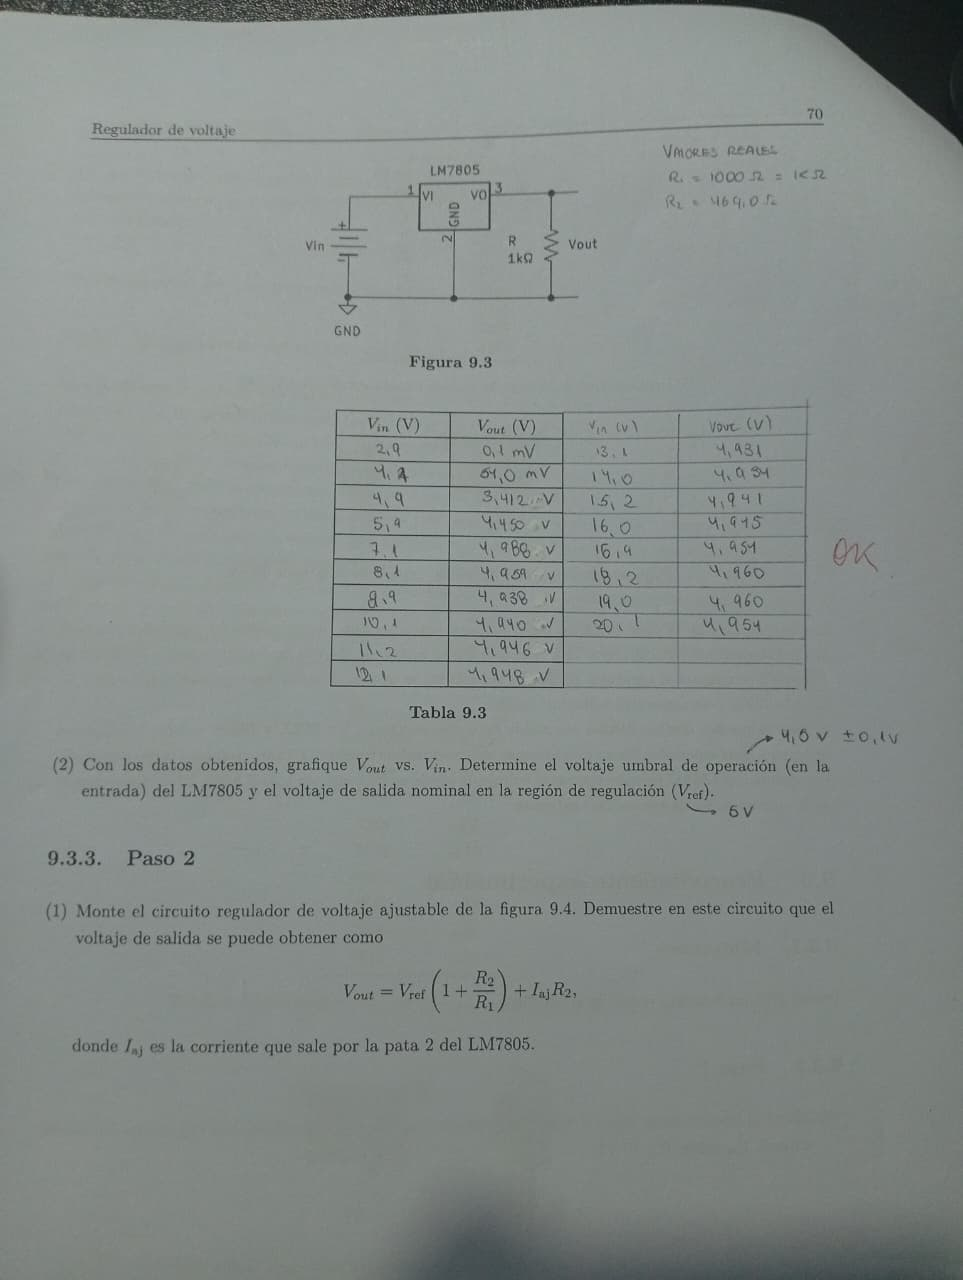
\includegraphics[width=\linewidth]{imagen5.jpeg}
        \caption{Anexo 1}
        \label{anexo1}
    \end{minipage}
    \hspace{0.02\linewidth}
    \begin{minipage}{0.48\linewidth}
        \centering
        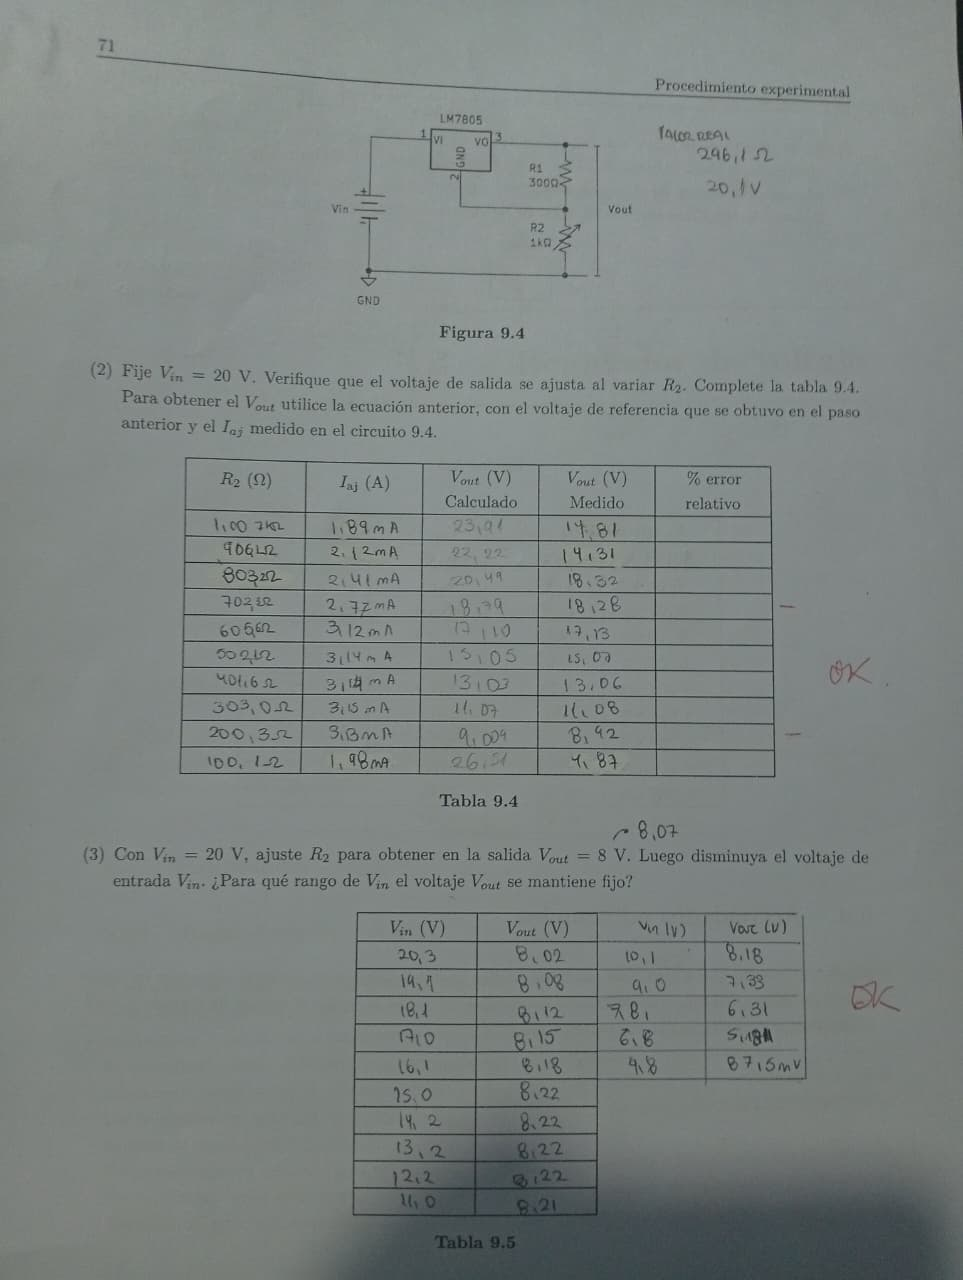
\includegraphics[width=\linewidth]{imagen6.jpeg}
        \caption{Anexo 2}
        \label{anexo2}
    \end{minipage}
\end{figure}

\begin{figure}[H]
    \centering
    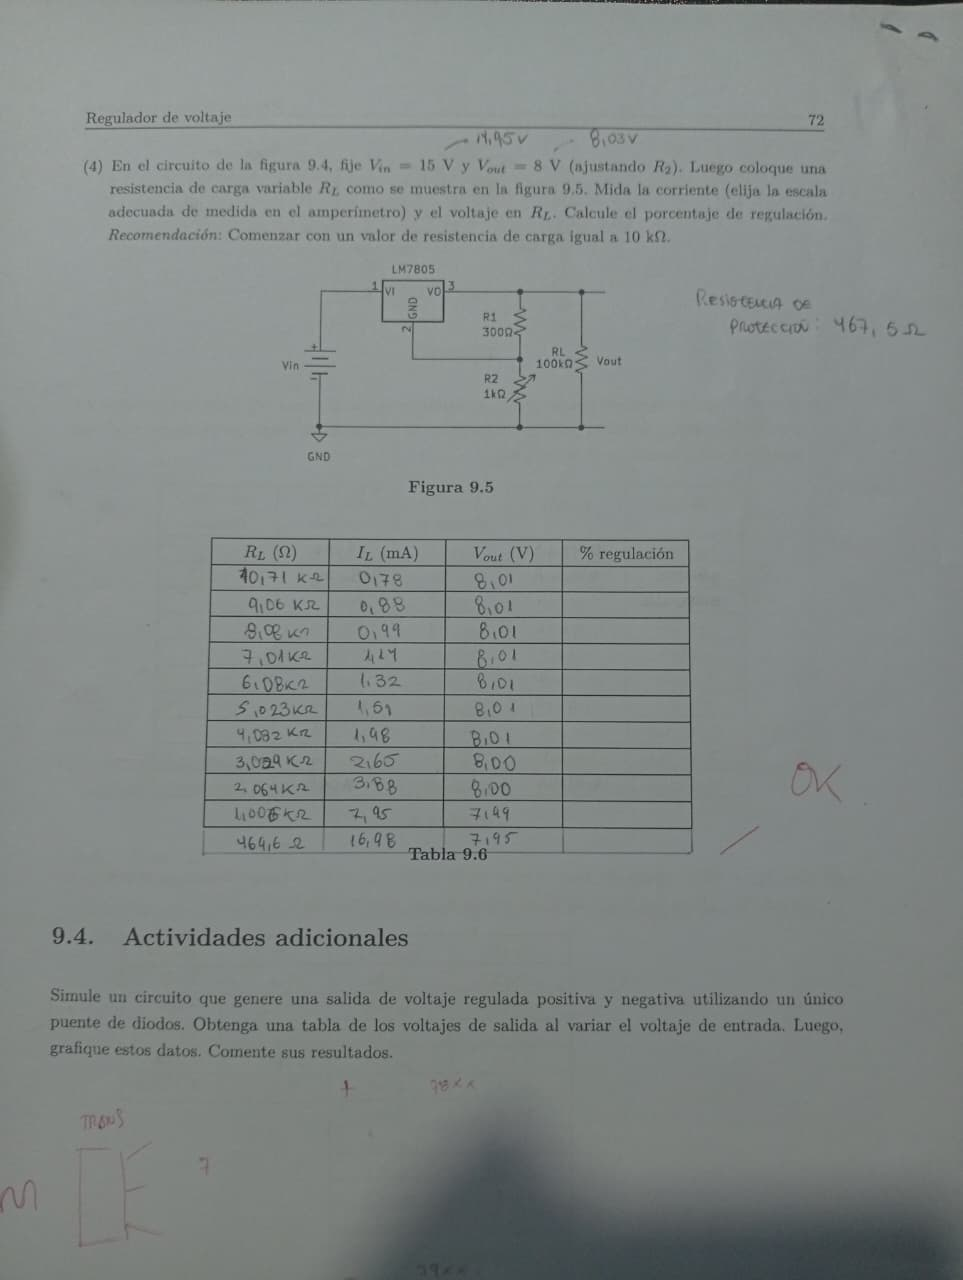
\includegraphics[width=0.6\linewidth]{imagen7.jpeg}
    \caption{Anexo 3}
    \label{anexo3}
\end{figure}

\end{document}

